\documentclass[11pt]{article}

\usepackage{epsfig}
\usepackage{amsfonts}
\usepackage{amssymb}
\usepackage{amstext}
\usepackage{amsmath}
\usepackage{xspace}
\usepackage{theorem}
\usepackage{color}
%\usepackage{times}
\usepackage{graphicx}
\usepackage{url}

%\usepackage{layout}% if you want to see the layout parameters
                     % and now use \layout command in the body

% This is the stuff for normal spacing
\makeatletter
 \setlength{\textwidth}{6.5in}
 \setlength{\oddsidemargin}{0in}
 \setlength{\evensidemargin}{0in}
 \setlength{\topmargin}{0.25in}
 \setlength{\textheight}{8.25in}
 \setlength{\headheight}{0pt}
 \setlength{\headsep}{0pt}
 \setlength{\marginparwidth}{59pt}

 \setlength{\parindent}{0pt}
 \setlength{\parskip}{5pt plus 1pt}
 \setlength{\theorempreskipamount}{5pt plus 1pt}
 \setlength{\theorempostskipamount}{0pt}
 \setlength{\abovedisplayskip}{8pt plus 3pt minus 6pt}

 \renewcommand{\section}{\@startsection{section}{1}{0mm}%
                                   {2ex plus -1ex minus -.2ex}%
                                   {1.3ex plus .2ex}%
                                   {\normalfont\Large\bfseries}}%
 \renewcommand{\subsection}{\@startsection{subsection}{2}{0mm}%
                                     {1ex plus -1ex minus -.2ex}%
                                     {1ex plus .2ex}%
                                     {\normalfont\large\bfseries}}%
 \renewcommand{\subsubsection}{\@startsection{subsubsection}{3}{0mm}%
                                     {1ex plus -1ex minus -.2ex}%
                                     {1ex plus .2ex}%
                                     {\normalfont\normalsize\bfseries}}
 \renewcommand{\paragraph}{\@startsection{paragraph}{4}{0mm}%
                                    {1ex \@plus1ex \@minus.2ex}%
                                    {-1em}%
                                    {\normalfont\normalsize\bfseries}}
 \renewcommand{\subparagraph}{\@startsection{subparagraph}{5}{\parindent}%
                                       {2.0ex \@plus1ex \@minus .2ex}%
                                       {-1em}%
                                      {\normalfont\normalsize\bfseries}}
\makeatother

\newenvironment{proof}{{\bf Proof:  }}{\hfill\rule{2mm}{2mm}}
\newenvironment{proofof}[1]{{\bf Proof of #1:  }}{\hfill\rule{2mm}{2mm}}
\newenvironment{proofofnobox}[1]{{\bf#1:  }}{}
\newenvironment{example}{{\bf Example:  }}{\hfill\rule{2mm}{2mm}}
%\renewcommand{\thesection}{\lecnum.\arabic{section}}

\renewcommand{\theequation}{\thesection.\arabic{equation}}
%\renewcommand{\thefigure}{\thesection.\arabic{figure}}
\renewcommand{\thefigure}{\arabic{figure}}

\newtheorem{fact}{Fact}[section]
\newtheorem{lemma}[fact]{Lemma}
\newtheorem{theorem}[fact]{Theorem}
\newtheorem{definition}[fact]{Definition}
\newtheorem{corollary}[fact]{Corollary}
\newtheorem{proposition}[fact]{Proposition}
\newtheorem{claim}[fact]{Claim}
\newtheorem{exercise}[fact]{Exercise}

% math notations
\newcommand{\R}{\ensuremath{\mathbb R}}
\newcommand{\Z}{\ensuremath{\mathbb Z}}
\newcommand{\N}{\ensuremath{\mathbb N}}
\newcommand{\F}{\ensuremath{\mathcal F}}
\newcommand{\SymGrp}{\ensuremath{\mathfrak S}}

\newcommand{\size}[1]{\ensuremath{\left|#1\right|}}
\newcommand{\ceil}[1]{\ensuremath{\left\lceil#1\right\rceil}}
\newcommand{\floor}[1]{\ensuremath{\left\lfloor#1\right\rfloor}}
\newcommand{\poly}{\operatorname{poly}}
\newcommand{\polylog}{\operatorname{polylog}}

% asymptotic notations
\newcommand{\Oh}[1]{{\mathcal O}\left({#1}\right)}
\newcommand{\LOh}[1]{{\mathcal O}\left({#1}\right.}
\newcommand{\ROh}[1]{{\mathcal O}\left.{#1}\right)}
\newcommand{\oh}[1]{{o}\left({#1}\right)}
\newcommand{\Om}[1]{{\Omega}\left({#1}\right)}
\newcommand{\om}[1]{{\omega}\left({#1}\right)}
\newcommand{\Th}[1]{{\Theta}\left({#1}\right)}


% pseudocode notations
\newcommand{\xif}{{\bf{\em{if~}}}}
\newcommand{\xthen}{{\bf{\em{then~}}}}
\newcommand{\xelse}{{\bf{\em{else~}}}}
\newcommand{\xelseif}{{\bf{\em{elif~}}}}
\newcommand{\xfi}{{\bf{\em{fi~}}}}
\newcommand{\xendif}{{\bf{\em{endif~}}}}
\newcommand{\xcase}{{\bf{\em{case~}}}}
\newcommand{\xendcase}{{\bf{\em{endcase~}}}}
\newcommand{\xbreak}{{\bf{\em{break~}}}}
\newcommand{\xfor}{{\bf{\em{for~}}}}
\newcommand{\xto}{{\bf{\em{to~}}}}
\newcommand{\xby}{{\bf{\em{by~}}}}
\newcommand{\xdownto}{{\bf{\em{downto~}}}}
\newcommand{\xdo}{{\bf{\em{do~}}}}
\newcommand{\xrof}{{\bf{\em{rof~}}}}
\newcommand{\xwhile}{{\bf{\em{while~}}}}
\newcommand{\xendwhile}{{\bf{\em{endwhile~}}}}
\newcommand{\xand}{{\bf{\em{and~}}}}
\newcommand{\xor}{{\bf{\em{or~}}}}
\newcommand{\xerror}{{\bf{\em{error~}}}}
\newcommand{\xreturn}{{\bf{\em{return~}}}}
\newcommand{\xparallel}{{\bf{\em{parallel~}}}}
\newcommand{\xspawn}{{\bf{\em{spawn~}}}}
\newcommand{\xsync}{{\bf{\em{sync~}}}}
\newcommand{\xarray}{{\bf{\em{array~}}}}
\newcommand{\T}{\hspace{0.5cm}}
\newcommand{\m}{\mathcal}

\def\sland{~\land~}
\def\slor{~\lor~}
\def\sRightarrow{~\Rightarrow~}

\definecolor{gray}{rgb}{0.3,0.3,0.3}

\def\comment#1{\hfill{\color{gray}{$\left\{\textrm{{\em{#1}}}\right\}$}}}
\def\lcomment#1{\hfill{\color{gray}{$\left\{\textrm{{\em{#1}}}\right.$}}}
\def\rcomment#1{\hfill{\color{gray}{$\left.\textrm{{\em{#1}}}\right\}$}}}
\def\fcomment#1{\hfill{\color{gray}{$\textrm{{\em{#1}}}$}}}
\def\func#1{\mbox{\textrm{\bf{\sc{#1}}}}}
\def\funcbf#1{\mbox{\textrm{\textbf{\textsc{#1}}}}}

\newcommand{\hide}[1]{}

\newcommand{\prob}[1]{\ensuremath{\text{{\bf Pr}$\left[#1\right]$}}}
\newcommand{\expct}[1]{\ensuremath{\text{{\bf E}$\left[#1\right]$}}}
\newcommand{\Event}{{\mathcal E}}

\newcommand{\mnote}[1]{\normalmarginpar \marginpar{\tiny #1}}

\makeatletter
   \newcommand\figcaption{\def\@captype{figure}\caption}
   \newcommand\tabcaption{\def\@captype{table}\caption}
\makeatother

 \def\para#1{\vspace{0.2cm}\noindent{\bf{#1.}}}

%%%%%%%%%%%%%%%%%%%%%%%%%%%%%%%%%%%%%%%%%%%%%%%%%%%%%%%%%%%%%%%%%%%%%%%%%%%
% Document begins here %%%%%%%%%%%%%%%%%%%%%%%%%%%%%%%%%%%%%%%%%%%%%%%%%%%%
%%%%%%%%%%%%%%%%%%%%%%%%%%%%%%%%%%%%%%%%%%%%%%%%%%%%%%%%%%%%%%%%%%%%%%%%%%%


\newcommand{\headings}[3]{
{\large
{\bf CSE638: Advanced Algorithms, Spring 2013} \hfill {{\bf Date:} #1}\vspace{-0.1cm}\\
\rule[0.01in]{\textwidth}{0.025in}}
%\hline
\begin{center} \vspace{-0.2cm}
{{\bf\huge{Homework \##2}}\\{\bf( Due: #3 )}} \end{center}
%\thispagestyle{empty}
}

\begin{document}

\headings{April 23}{3}{May 10}
\newcommand{\lecnum}{5}  % Lecture Number



\vspace{-0.5cm}
\para{Task 1} {\bf{[ 130 Points ]}} {\bf Matrix Multiplication.}
%
 \begin{itemize}

\vspace{-0.2cm}
 \item[$(a)$] {\bf{[ 20 Points ]}} Figure \ref{fi:iter-mm} shows the
 standard iterative matrix multiplication algorithm and its 5 variants
 obtained by permuting the three nested \xfor loops in all possible ways.
 Assuming that all three matrices ($X$, $Y$ and $Z$) are given in row-major
 order, analyze the cache complexity of each of the 6 versions of the
 algorithm. 

\vspace{-0.2cm}
 \item[$(b)$] {\bf{[ 30 Points ]}} Implement the cache-oblivious recursive
 matrix multiplication algorithm discussed in the class (\func{Rec-MM}
 in Lecture 15). But do not recurse down to matrices of size $1 \times 1$.
 Instead stop at a base case of size $m \times m$ for some $m > 0$ in order
 to reduce the overhead of recursion. When you reach a base case
 of size $m \times m$ use one of the most cache-efficient
 iterative algorithms for part $1(a)$ for multiplying the
 two subatrices. For simplicity let's assume that
 both $n$ and $m$ are powers of 2. For $n = 2^{13}$, empirically
 find the value of $m$ that gives you the smallest running
 time for \func{Rec-MM}. Produce a table or a graph showing
 how the running time varies as you change $m$.

\vspace{-0.2cm}
 \item[$(c)$] {\bf{[ 10 Points ]}} Analyze the running time and
 cache-complexity of the recursive divide-and-conquer algorithm
 (discussed in the class) that converts a matrix from row-major 
 layout to $Z$-Morton layout. Assume that $n$ is a power of 2.
 Argue that conversion from $Z$-Morton layout to row-major layout 
 has the same complexity.

\vspace{-0.2cm}
 \item[$(d)$] {\bf{[ 30 Points ]}} Consider the divide-and-conquer 
 algorithm from part $1(c)$ that converts from row-major to
 $Z$-Morton layout. Suppose instead of recursing down
 to matrices of size $1 \times 1$, we stop when we reach matrices
 of size $m \times m$ for some $m > 0$, and copy the entries
 from the input submatrix of size $m \times m$ to the output
 submatrix in row-major order. Similarly, for the algorithm
 that converts from $Z$-Morton to row-major. Let's call these
 two functions \func{R2Z} and \func{Z2R}, respectively. Now modify
 \func{Rec-MM} from part $1(b)$ to \func{Rec-MM-2} so that
 \func{Rec-MM-2} works correctly on a matrix in the 
 hybrid row-major-$Z$-Morton layout described above. Note 
 that the base case size of \func{Rec-MM-2} and the conversion 
 routines must match. We assume for simplicity that
 both $n$ and $m$ are powers of 2. For $n = 2^{13}$, empirically
 optimize the value of $m$ for \func{Rec-MM-2} as you did
 for \func{Rec-MM} in part $1(b)$. However, this time
 include the running times of \func{R2Z} that puts the input 
 matrices in the $Z$-Morton layout, and of \func{Z2R} that converts
 the output matrix back to row-major layout. Produce a table or a graph showing
 how the running time varies as you change $m$.

\vspace{-0.2cm}
 \item[$(e)$] {\bf{[ 40 Points ]}} Run all your matrix multiplication
 implementations from parts $1(a)$, $1(b)$ and $1(d)$ (parts $1(b)$ and $1(d)$
 with optimized base) to produce five tables: running times, instructions excuted,
 L1 misses, L2 misses and L3 misses. In each table create a row for each
 $n = 2^t$, $8 \leq t \leq 15$, and in each row include the corresponding
 figures for each of your implementations. Create two columns
 for \func{Rec-MM-2}: one including the cost of layout conversion
 and the other without that cost. Use {\tt PAPI}\footnote{To load 
 {\tt PAPI} use ``module load papi/4.1.2.1'' on {\tt Loanstar}.
 Check \url{http://icl.cs.utk.edu/papi/} for usage.}
 to find the number of L1, L2 and L3 misses as well as the
 number of instructions executed. Explain your findings.

 \end{itemize}


\para{Task 2} {\bf{[ 70 Points ]}} {\bf Protein Accordion Folding.}
%

A protein can be viewed as a string $\m{P}[1 : n]$ over the
alphabet \{ {\em A, R, N, D, C, E, Q, G, H, I, L, K, M, F, P, S, T, W, Y, V } \}
of amino acids\footnote{Amino acids: Alanine (A), Arginine (R), Asparagine (N),
Aspartic acid (D), Cysteine (C), Glutamic acid (E), Glutamine (Q), Glycine (G),
Histidine (H), Isoleucine (I), Leucine (L), Lysine (K), Methionine (M),
Phenylalanine (F), Proline (P), Serine (S), Threonine (T), Tryptophan (W),
Tyrosine (Y), Valine (V).}. A protein sequence is never straight, and instead
it folds itself in a way that minimizes the potential energy. Some of the amino 
acids (e.g., {\em A, I, L, F, G, P, V})\footnote{Alanine (A), Isoleucine (I), 
Leucine (L), Phenylalanine (F), Glycine (G), Proline (P), Valine (V).} are 
called {\em hydrophobic} as they do not like to be in contact with water (solvent).
A desire to minimize the total hydrophobic area exposed to water is a major driving force 
behind the folding process. In a folded protein hydrophobic amino acids
tend to clump together in order to reduce water-exposed hydrophobic area.

For simplicity, in this problem, we assume that a protein is folded into a 2D square lattice
in such a way that the number of pairs of hydrophobic amino acids that are next to each other 
in the grid (vertically or horizontally) without being next to each other in the protein
sequence is maximized. We also assume that the fold is always an {\em accordion fold} where the sequence first
goes straight down, then straight up, then again straight down, and so on (see Figure \ref{fig:fold}).

\begin{figure}[h]
	\centering
	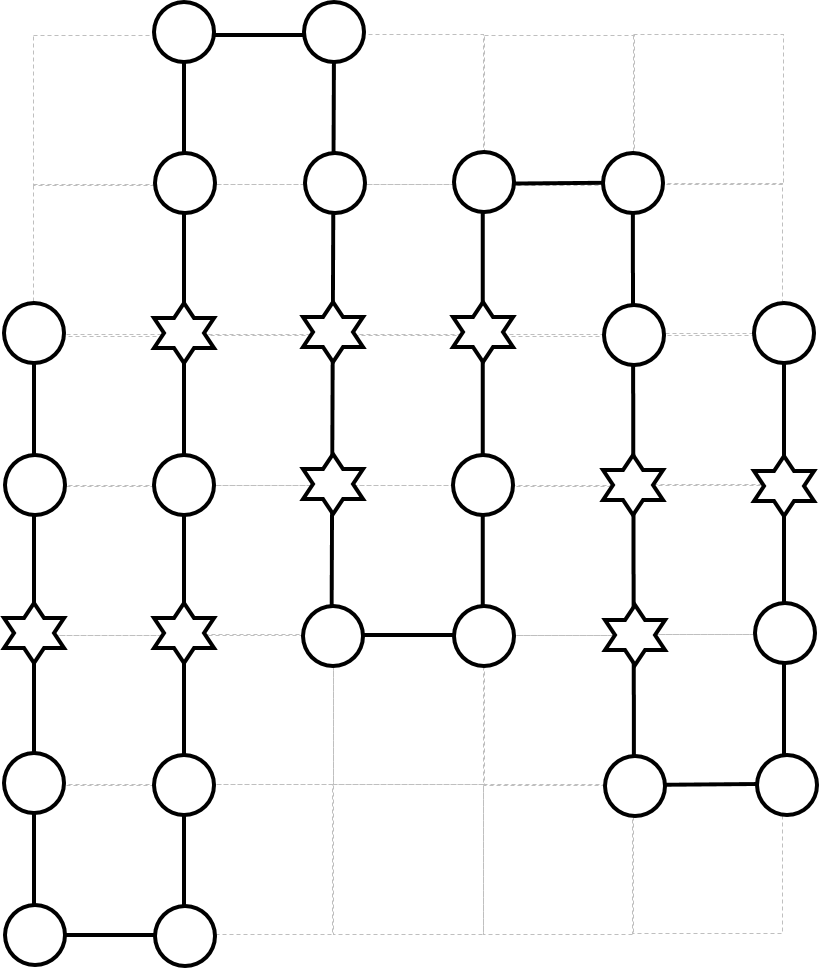
\includegraphics[scale=0.35]{protein-accordion-fold.png}
        \vspace{-0.3cm}
	\caption{A protein accordion fold where each star represents a hydrophobic amino acid and each circle a hydrophilic one. 
                 The accordion score of this folded sequence is 4 which is not the maximum possible accordion score for this sequence.}
	\label{fig:fold}
\end{figure}


The recurrence below shows how to compute the optimal {\em accordion acore} of the
protein segment $\m{P}[i:j]$. The optimal accordion score is given by $\max_{1 < j \leq n}{\left\{ \func{Score}(1, j) \right\}}$.

{
 \vspace{-0.2cm}
 \begin{eqnarray*}
\label{eq:score}
 \func{Score}( i, j ) = \left\{ \begin{array}{@{}l@{~}l}
                   0 & \textrm{if $j \geq n - 1$,}\\
                   \max_{j + 1 < k \leq n}{\left\{ \func{Score-One-Fold}( i, j, k ) + \func{Score}(j + 1, k) \right\} }~
                     & \textrm{otherwise}.
                   \end{array} \right.
 \end{eqnarray*}
}

The function \func{Score-One-Fold}$( i, j, k )$ counts the number of aligned hydrophobic amino acids when the
protein segment $\m{P}[i:k]$ is folded only once at indices $(j, j+ 1)$. The function is
given in Figure \ref{fi:score-one-fold}, and illustrated graphically in Figure \ref{fig:one-fold}.

\begin{figure}[h]
	\centering
	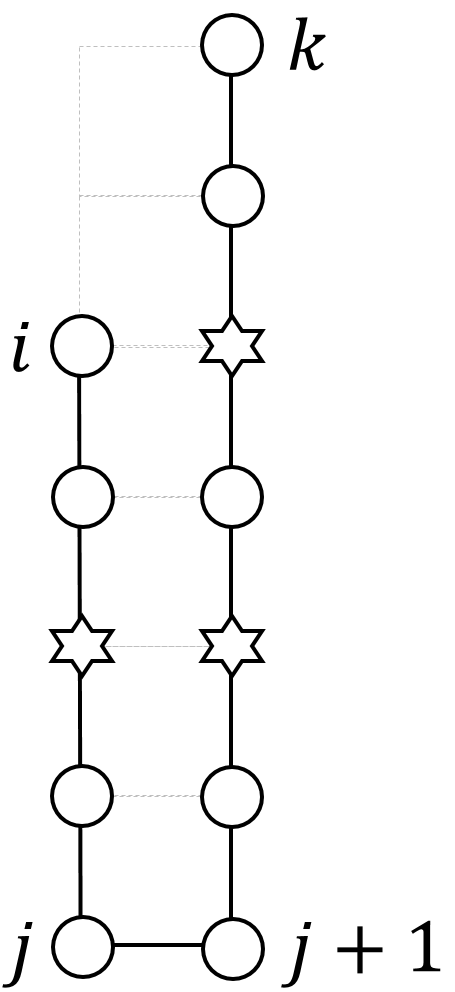
\includegraphics[scale=0.3]{score-one-fold.png}
        \vspace{-0.3cm}
	\caption{\func{Score-One-Fold}( i, j, k ) counts the number of aligned hydrophobic amino acids when the
protein segment $\m{P}[i:k]$ is folded only once at indices $(j, j+ 1)$. In this figure,
each star represents a hydrophobic amino acid and each circle a hydrophilic one.}
	\label{fig:one-fold}
\end{figure}




\begin{itemize}

    \item[$(a)$] {\bf{[ 5 Points ]}} Show that a straightforward iterative implementation 
        of the recurrence for \func{Score} runs in $\Oh{n^4}$ time and uses $\Th{n^2}$ space.

    \item[$(a)$] {\bf{[ Answer: ]}}
        \begin{verbatim}
//Runs in O(n^4) time (O(n^3) * O(n)) and uses O(n^2) space.
OptimalScore_A(P[1:n]) {
    for i := n downto 1 {
        for j := n downto i+1 {
            if j >= n-1 {
                Score(i, j) := 0;
            } else {
                best := 0;
                for k := n downto j+2 {
                    candidate := ScoreOneFold_A(i, j, k) + Score(j+1, k);
                    best := max(candidate, best);
                }
                Score(i, j) := best;
            }
        }
    }
    answer := 0;
    for j := 1 to n {
        answer := max(answer, Score(1, j);
    }
    return answer;
}

//Runs in O(n) time and uses O(1) space.
ScoreOneFold_A(i, j, k, P[1:n]) {
    c := 0;
    for l := 1 to min(j-i, k-j-1) {
        if Hydrophobic(P[j-l]) and Hydrophobic(P[j+1+l]) {
            c := c + 1;
        }
    }
    return c;
}
        \end{verbatim}

    \item[$(b)$] {\bf{[ 5 Points ]}} Explain how to modify the implementation from part 
        $2(a)$ to run in $\Oh{n^3}$ time at the cost of increasing the space complexity to $\Th{n^3}$.
        Analyze its cache-complexity. 

    \item[$(b)$] {\bf{[ Answer: ]}}
        Precompute the $\Oh{n^3}$ possible answers for \func{ScoreOneFold} and store them in $\Oh{n^3}$ space.
        We assume $\alpha M>n$ (we can store at least a constant number of rows of size $n$ in memory).
        This is similar to (c) for cache complexity, except for reading and writing to ScoreOneFold.
        Cost to read it during processing and write during preprocessing is $\Oh{\frac{n^3}{B}}$ cache-misses.
        Total cost is $\Oh{\frac{n^3}{B}}$ cache-misses, which is optimal because there is no room to improve due to temporal locality (space is $\Theta$ of time.

        \begin{verbatim}
//Runs in O(n^3) time and uses O(n^3) space.
OptimalScore_B(P[1:n]) {
    ScoreOneFold[][][] = ScoreOneFold_B(P); //Generate all n^3 answers.
    for i := n downto 1 {
        for j := n downto i+1 {
            if j >= n-1 {
                Score(i, j) := 0;
            } else {
                best := 0;
                for k := n downto j+2 {
                    candidate := ScoreOneFold[i][j][k] + Score(j+1, k);
                    best := max(candidate, best);
                }
                Score(i, j) := best;
            }
        }
    }
    answer := 0;
    for j := 1 to n {
        answer := max(answer, Score(1, j);
    }
    return answer;
}

//Runs in O(n^3) time and uses O(n^3) space.
ScoreOneFold_B(P[1:n]) {
    int ScoreOneFold[n][n][n];
    int ScoreOneFold_2[n][n] = ScoreOneFold_C(P);
    for i := 1 to n {
        for j := 1 to n {
            for k := 1 to n {
                l := min(j-i, k-j-1);
                ScoreOneFold[i][j][k] := ScoreOneFold_2[j][l];
            }
        }
    }
    return ScoreOneFold;
}
        \end{verbatim}

    \item[$(c)$] {\bf{[ 10 Points ]}} Show that the space usage of the implementation from 
        part $2(b)$ can be reduced to $\Oh{n^2}$ without increasing its running time.
        Analyze its cache-complexity.

    \item[$(c)$] {\bf{[ Answer: ]}}
        Part (b) above can be improved by realizing the redundancy.  The redundancy is explicitly shown above in \func{ScoreOneFold\_B}.
        We assume $\alpha M>n$ (we can store at least a constant number of rows of size $n$ in memory).
        For each $1\leq i\leq n$, we read all lower rows costing $\Oh{\frac{n^2}{B}}$ cache-misses each.  Total cost is $\Oh{\frac{n^3}{B}}$ cache-misses.  Other parts are dominated by this. There is (at least the potential for) room for improvement due to temporal locality because the space is asymptotically smaller than time.

        \begin{verbatim}
//Runs in O(n^3) time and uses O(n^2) space.
OptimalScore_C(P[1:n]) {
    ScoreOneFold[][] = ScoreOneFold_C(P); //Generate all n^3 answers.
    for i := n downto 1 {
        for j := n downto i+1 {
            if j >= n-1 {
                Score(i, j) := 0;
            } else {
                best := 0;
                for k := n downto j+2 {
                    l := min(j-i, k-j-1);
                    candidate := ScoreOneFold[j][l] + Score(j+1, k);
                    best := max(candidate, best);
                }
                Score(i, j) := best;
            }
        }
    }
    answer := 0;
    for j := 1 to n {
        answer := max(answer, Score(1, j);
    }
    return answer;
}

//Runs in O(n^2) time and uses O(n^2) space.
ScoreOneFold_C(P[1:n]) {
    int ScoreOneFold[n][n];
    for j:= 1 to n {
        max_l := min(j-1, n-j-1);
        for l := 0 to n {
            if l < 1 {
                ScoreOneFold[j][l] := 0;
            } else if l > max_l {
                ScoreOneFold[j][l] := ScoreOneFold[j][max_l];
            } else if Hydrophobic(P[j-l]) and Hydrophobic(P[j+1+l]) {
                ScoreOneFold[j][l] := ScoreOneFold[j][l-1] + 1;
            } else {
                ScoreOneFold[j][l] := ScoreOneFold[j][l-1];
            }
        }
    }
    return ScoreOneFold;
}
        \end{verbatim}

    \item[$(d)$] {\bf{[ 50 Points ]}} Convert your iterative algorithm from part $2(c)$
        into a recursive divide-and-conquer algorithm that runs in $\Oh{n^3}$ time, uses
        $\Oh{n^2}$ space, and incurs only $\Oh{{n^3 \over {B\sqrt{M}}}}$ cache-misses,
        where $M$ is the size of the cache and $B$ is the block transfer size. 
        Explain why the algorithm from part $2(b)$ cannot be converted
        in the same way\footnote{convert to a recursive divide-and-conquer algorithm
            without changing the time and space complexities of the
        iterative algorithm} to achieve the same aymptotic cache-complexity.

    \item[$(d)$] {\bf{[ Answer: ]}}
        $2(b)$ cannot be changed to achieve the same complexity because the complexity is optimal for the given running time and space usage.

        \func{ScoreOneFold\_C} can be turned to divide and conquer:
        \begin{verbatim}
OptimalScore_D(P[1:n]) {
    ScoreOneFold[][] = ScoreOneFold_C(P); //Generate all n^3 answers.
    Score[][];
    OptimalScore_D_Recur(P, n, 1, 1, Score, ScoreOneFold);

    answer := 0;
    for j := 1 to n {
        answer := max(answer, Score(1, j);
    }
    return answer;
}

OptimalScore_D_Recur(P[1:n], size, i, j, Score[][], ScoreOneFold[][]) {
    if size == 1 {
        best := 0;
        for k := n downto j+2 {
            l := min(j-i, k-j-1);
            candidate := ScoreOneFold[j][l] + Score(j+1, k);
            best := max(candidate, best);
        }
        Score(i, j) := best;
    } else {
        OptimalScore_D(P, size/2, i + size/2, j + size/2, Score, ScoreOneFold);
        OptimalScore_D(P, size/2, i + size/2, j,          Score, ScoreOneFold);
        OptimalScore_D(P, size/2, i,          j + size/2, Score, ScoreOneFold);
        OptimalScore_D(P, size/2, i,          j,          Score, ScoreOneFold);
    }
}
        \end{verbatim}

\end{itemize}


\begin{figure*}[h!]
% \vspace{0.8cm}
 \begin{minipage}{\textwidth}
 \begin{center}
 \framebox{
 \begin{minipage}{\textwidth}
 {\footnotesize
 \medskip\noindent\func{Score-One-Fold}$(~i, ~j, ~k,~ {\m{P}} ~)$

 \vspace{0.1cm}
 \noindent
 ({\color{gray} ${\m{P}}[1:n]$ is a sequence of amino acids, where $n > k - 1 > j > i > 0$. 
 This function counts the number of aligned hydrophobic pairs when the segment
 ${\m{P}}[i:k]$ is folded at locations $j$ and $j + 1$.})

 \noindent
 \begin{enumerate}

 \item $c \gets 0$

 \item \xfor $l \gets 1$ \xto $\min{\left(~ j - i,~ k - j - 1~ \right)}$ \xdo

 \item \T \xif \func{Hydrophobic}$(~{\m{P}}[j - l]~)$ \xand \func{Hydrophobic}$(~{\m{P}}[j + 1 + l]~)$ \xthen $c \gets c + 1$

 \item \xreturn $c$

 \vspace{0.2cm}

 \end{enumerate}
 }
 \end{minipage}
 }
 \vspace{-0.3cm}
 \caption{Count the number of aligned hydrophobic amino acids when a protein sequence is folded once.}
 \label{fi:score-one-fold}
 \vspace{-0.3cm}
 \end{center}
 \end{minipage}
 \end{figure*}


\newpage
\begin{figure*}[hp!]
% \vspace{0.8cm}
 \begin{minipage}{\textwidth}
 \begin{center}
 \framebox{
 \begin{minipage}{\textwidth}
 {\footnotesize
 \medskip\noindent\func{Iter-MM-ijk}$(~Z, ~X, ~Y, ~n ~)$

 \vspace{0.1cm}
 \noindent
 ({\color{gray} Inputs are three $n \times n$ matrices $X$, $Y$
 and $Z$. For each $i, j \in [1, n]$, 
 $Z[ i, j ]$ is set to $Z[ i, j ] + \sum_{k = 1}^{n}{X[ i, k ] \times Y[ k, j ]}$.})

 \noindent
 \begin{enumerate}

 \item \xfor $i \gets 1$ \xto $n$ \xdo

 \item \T \xfor $j \gets 1$ \xto $n$ \xdo

 \item \T\T \xfor $k \gets 1$ \xto $n$ \xdo

 \item \T\T\T $Z[ i, j ] \gets Z[ i, j ] + X[ i, k ] \times Y[ k, j ]$

 \vspace{0.1cm}

 \end{enumerate}

 }
 \end{minipage}
 \vspace{0.1cm}
 }

 \framebox{
 \begin{minipage}{\textwidth}
 {\footnotesize
 \medskip\noindent\func{Iter-MM-ikj}$(~Z, ~X, ~Y, ~n ~)$

 \vspace{0.1cm}
 \noindent
 ({\color{gray} Inputs are three $n \times n$ matrices $X$, $Y$
 and $Z$. For each $i, j \in [1, n]$, 
 $Z[ i, j ]$ is set to $Z[ i, j ] + \sum_{k = 1}^{n}{X[ i, k ] \times Y[ k, j ]}$.})

 \noindent
 \begin{enumerate}

 \item \xfor $i \gets 1$ \xto $n$ \xdo

 \item \T \xfor $k \gets 1$ \xto $n$ \xdo

 \item \T\T \xfor $j \gets 1$ \xto $n$ \xdo

 \item \T\T\T $Z[ i, j ] \gets Z[ i, j ] + X[ i, k ] \times Y[ k, j ]$

 \vspace{0.1cm}

 \end{enumerate}

 }
 \end{minipage}
 \vspace{0.1cm}
 }

 \framebox{
 \begin{minipage}{\textwidth}
 {\footnotesize
 \medskip\noindent\func{Iter-MM-jik}$(~Z, ~X, ~Y, ~n ~)$

 \vspace{0.1cm}
 \noindent
 ({\color{gray} Inputs are three $n \times n$ matrices $X$, $Y$
 and $Z$. For each $i, j \in [1, n]$, 
 $Z[ i, j ]$ is set to $Z[ i, j ] + \sum_{k = 1}^{n}{X[ i, k ] \times Y[ k, j ]}$.})

 \noindent
 \begin{enumerate}

 \item \xfor $j \gets 1$ \xto $n$ \xdo

 \item \T \xfor $i \gets 1$ \xto $n$ \xdo

 \item \T\T \xfor $k \gets 1$ \xto $n$ \xdo

 \item \T\T\T $Z[ i, j ] \gets Z[ i, j ] + X[ i, k ] \times Y[ k, j ]$

 \vspace{0.1cm}

 \end{enumerate}

 }
 \end{minipage}
 \vspace{0.1cm}
 }

 \framebox{
 \begin{minipage}{\textwidth}
 {\footnotesize
 \medskip\noindent\func{Iter-MM-jki}$(~Z, ~X, ~Y, ~n ~)$

 \vspace{0.1cm}
 \noindent
 ({\color{gray} Inputs are three $n \times n$ matrices $X$, $Y$
 and $Z$. For each $i, j \in [1, n]$, 
 $Z[ i, j ]$ is set to $Z[ i, j ] + \sum_{k = 1}^{n}{X[ i, k ] \times Y[ k, j ]}$.})

 \noindent
 \begin{enumerate}

 \item \xfor $j \gets 1$ \xto $n$ \xdo

 \item \T \xfor $k \gets 1$ \xto $n$ \xdo

 \item \T\T \xfor $i \gets 1$ \xto $n$ \xdo

 \item \T\T\T $Z[ i, j ] \gets Z[ i, j ] + X[ i, k ] \times Y[ k, j ]$

 \vspace{0.1cm}

 \end{enumerate}

 }
 \end{minipage}
 \vspace{0.1cm}
 }

 \framebox{
 \begin{minipage}{\textwidth}
 {\footnotesize
 \medskip\noindent\func{Iter-MM-kij}$(~Z, ~X, ~Y, ~n ~)$

 \vspace{0.1cm}
 \noindent
 ({\color{gray} Inputs are three $n \times n$ matrices $X$, $Y$
 and $Z$. For each $i, j \in [1, n]$, 
 $Z[ i, j ]$ is set to $Z[ i, j ] + \sum_{k = 1}^{n}{X[ i, k ] \times Y[ k, j ]}$.})

 \noindent
 \begin{enumerate}

 \item \xfor $k \gets 1$ \xto $n$ \xdo

 \item \T \xfor $i \gets 1$ \xto $n$ \xdo

 \item \T\T \xfor $j \gets 1$ \xto $n$ \xdo

 \item \T\T\T $Z[ i, j ] \gets Z[ i, j ] + X[ i, k ] \times Y[ k, j ]$

 \vspace{0.1cm}

 \end{enumerate}

 }
 \end{minipage}
 \vspace{0.1cm}
 }

 \framebox{
 \begin{minipage}{\textwidth}
 {\footnotesize
 \medskip\noindent\func{Iter-MM-kji}$(~Z, ~X, ~Y, ~n ~)$

 \vspace{0.1cm}
 \noindent
 ({\color{gray} Inputs are three $n \times n$ matrices $X$, $Y$
 and $Z$. For each $i, j \in [1, n]$, 
 $Z[ i, j ]$ is set to $Z[ i, j ] + \sum_{k = 1}^{n}{X[ i, k ] \times Y[ k, j ]}$.})

 \noindent
 \begin{enumerate}

 \item \xfor $k \gets 1$ \xto $n$ \xdo

 \item \T \xfor $j \gets 1$ \xto $n$ \xdo

 \item \T\T \xfor $i \gets 1$ \xto $n$ \xdo

 \item \T\T\T $Z[ i, j ] \gets Z[ i, j ] + X[ i, k ] \times Y[ k, j ]$

 \vspace{0.1cm}

 \end{enumerate}

 }
 \end{minipage}
 \vspace{0.1cm}
 }


 \vspace{-0.2cm}
 \caption{Standard iterative matrix multiplication algorithm and its variants.}
 \label{fi:iter-mm}
 \vspace{-0.3cm}
 \end{center}
 \end{minipage}
 \end{figure*}



\newpage


\vspace{2cm}

\section*{APPENDIX 1: What to Turn in}

 One compressed archive file (e.g., zip, tar.gz) containing the following items.
%
 \begin{itemize}
%
\vspace{-0.1cm}
 \item[--] Source code, makefiles and job scripts.
%
\vspace{-0.1cm}
 \item[--] A PDF document containing all answers and plots.
%
 \end{itemize}


\section*{APPENDIX 2: Things to Remember}
%
 \begin{itemize}
%
\vspace{-0.1cm}
 \item[--] {\bf Please never run anything that takes more than a minute or uses multiple cores on TACC login nodes.}
          TACC policy strictly prohibits such usage. They reserve the right to suspend your account if you
          do so. All runs must be submitted as jobs to compute nodes (even when you use Cilkview or PAPI).
%
\vspace{-0.1cm}
 \item[--] Please store all data in your work folder (\$WORK), and not in your home folder (\$HOME).
%
\vspace{-0.1cm}
 \item[--] When measuring running times please exclude the time needed for reading the input and writing
          the output. Measure only the time needed by the algorithm. Do the same thing when you
          use PAPI.
%
 \end{itemize}


\end{document}



